

\begin{frame}
    \frametitle{Определение}
    \begin{description}
        \item[Геоданные:] данные о пространственных объектах и явлениях.
        \item[Пространственный объект:] цифровая модель материального или абстрактного объекта реального или виртуального мира включающая его идентификаторы, координатные и атрибутивные данные.
    \end{description}
\end{frame}

\begin{frame}
    \frametitle{Особенности пространственных данных.}
    \begin{itemize}
        \item геопространственные системы координат
        \item высокая информационная насыщенность
        \item объединение геометрической и атрибутивной информации
        \item послойная организация
    \end{itemize}
\end{frame}

\begin{frame}
    \frametitle{Явное нахождение в одной и пространственных систем координат.}
    \begin{multicols}{2}
       \begin{figure}[!ht]
           \begin{center}
               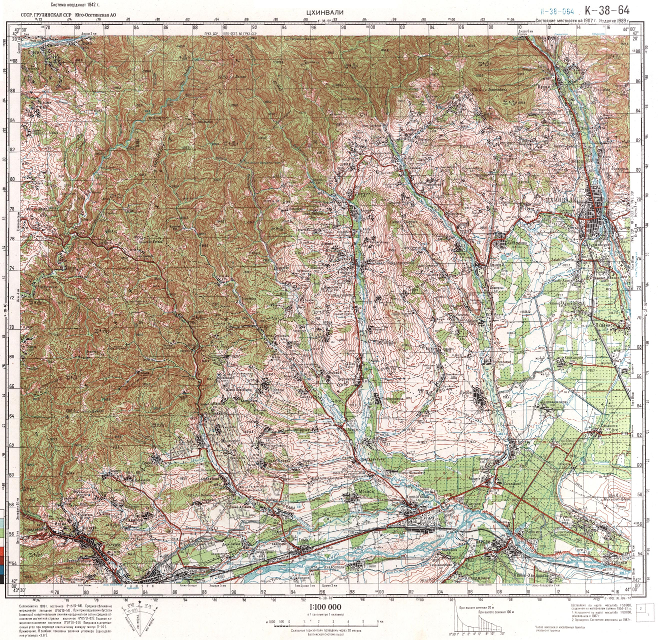
\includegraphics[width=0.8\columnwidth]{./introduction/img/topo_map}
           \end{center}
           \caption{Отсканированное изображение, каждый элемент имеет X,Y,Z}
       \end{figure}

       \begin{figure}[!ht]
           \begin{center}
               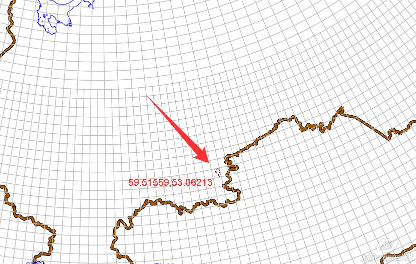
\includegraphics[width=0.95\columnwidth]{./introduction/img/grid_map}
           \end{center}
           \caption{Географически привязанное изображение, каждый элемент имеет широту, долготу, Z}
       \end{figure}
    \end{multicols}
\end{frame}

\begin{frame}
    \frametitle{Высокая информационная насыщенность}
    \begin{description}
        \item[MODIS] Передача 10.6 миллионов бит данных в секунду, т.е. около 53 Тб данных в день.
        \item[OpenStreetMap] (на начало ноября 2014):
            \begin{itemize}
                \item Число пользователей: 1.85 миллиона;
                \item Число узлов: 2597 миллионов;
                \item Число загруженных точек GPS: 4384 миллионов.
            \end{itemize}
    \end{description}
\end{frame}

\begin{frame}
    \frametitle{Послойная организация}
    \begin{figure}[!ht]
        \begin{center}
            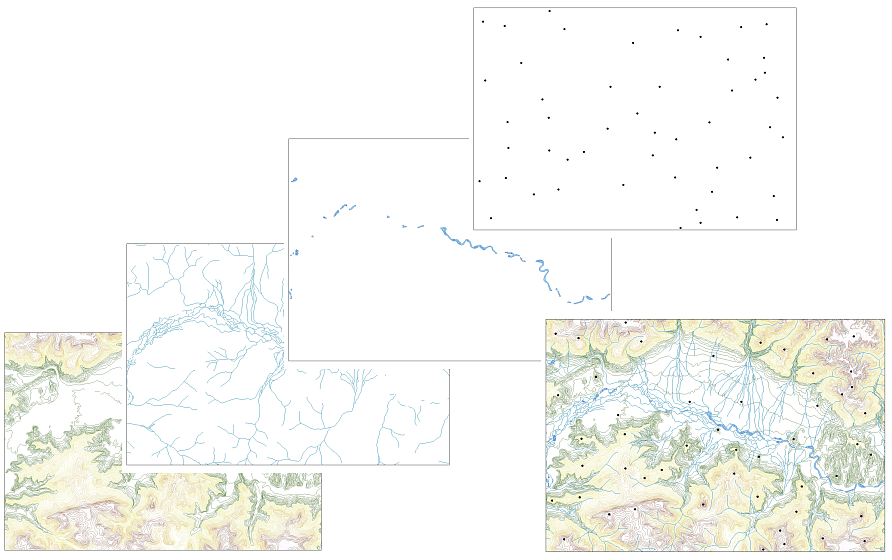
\includegraphics[width=0.9\columnwidth]{./introduction/img/layers_map}
        \end{center}
    \end{figure}
\end{frame}


\begin{frame}
    \frametitle{Объединение геометрической и атрибутивной информации}
    \begin{figure}[!ht]
        \begin{center}
            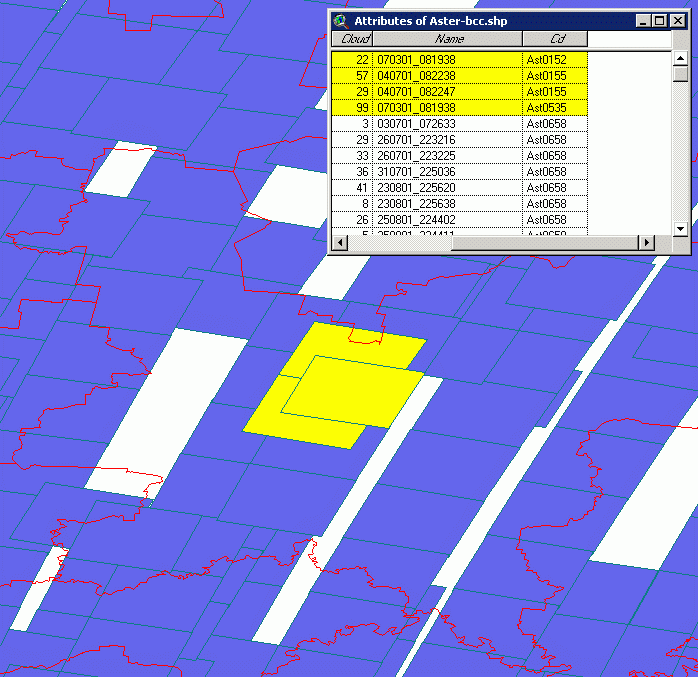
\includegraphics[width=0.55\columnwidth]{./introduction/img/attributes_and_geo}
        \end{center}
    \end{figure}
    Каждый элемент геометрии связан с набором атрибутивных полей (shape --- простая таблица, sqlite/spatialite, PodtgreSQL/PostGIS --- полноценная БД).
\end{frame}


\begin{frame}
    \frametitle{Типы данных}
    Два основных представления данных в ГИС:
    \begin{itemize}
        \item Векторный: обычно используется для представления дискретных объектов, имеющих четкие границы (в масштабе задачи). Например, домов, дорог, озер, \dots
        \item Растровый: часто используется для представления непрерывных объектов и явлений, но может использоваться и для представления дискретных объектов. Основное требование к растровому представлению данных --- размер ячейки должен быть
        значительно меньше, чем размеры объектов.
    \end{itemize}
\end{frame}

